\subsection{Instrument failures}
\label{sec:failures}

Seven failures of the instrument share a shape: it answered successfully, and answered about
something else. Table~\ref{tab:failures} lists them and Figure~\ref{fig:architecture} marks each on
the topology. The first four crossed a boundary with another server. The last three are ours, two in
the analysis code that produces our results and one in the pipeline that produces the artefact the
analyst receives, so the shape stops neither at the network boundary nor at the evaluation harness.

\begin{table}[!htbp]
\caption{The seven instrument failures, with the layer each occurred at and what found it.}\label{tab:failures}
\centering\small
\begin{tabular}{@{}
  >{\raggedright\arraybackslash}p{0.05\linewidth}
  >{\raggedright\arraybackslash}p{0.38\linewidth}
  >{\raggedright\arraybackslash}p{0.18\linewidth}
  >{\raggedright\arraybackslash}p{0.24\linewidth}@{}}
\toprule
& what the instrument did & layer & what found it \\
\midrule
M1 & an optional argument the agent never supplied arrived as an explicit \texttt{null}, and a field typed \texttt{str} rejected it, failing all \fact{cape-tool-count} tools & sandbox MCP client & every call returning the same validation error \\
M2 & \texttt{load\_program} answered \texttt{success} without changing the server's current program, so everything derived from it described the first binary of that container's lifetime & reverse-engineering server session state & call graphs identical to the character across unrelated samples \\
M3 & a load the server could not perform answered HTTP~200 with an error in the body, so downstream code analysed whichever program remained current & HTTP status against body & \fact{stuck-graph-run} consecutive samples at exactly \fact{stuck-graph-chars} characters \\
M4 & a \fact{react-step-budget}-step ReAct budget and a wall-clock cap composed into a path that returned zero techniques, at \fact{m4-total-minutes} minutes per attempt & two local bounds & a \fact{m4-salvage-minutes}-minute call always producing one claim and zero techniques \\
M5 & an ablation varied a deterministic reconciliation step and the output was attributed to a language model & our analysis code & a Jaccard too clean for a model to produce \\
M6 & a rank correlation over model size ranked a reasoning-configuration flag instead, recovering the published scaling coefficient & our analysis code & reading the arms table under the correlation \\
M7 & a documented output ceiling was renamed during serialisation to a key the server does not read, so a component described as bounded was never bounded & our production pipeline & a study recording which failure branch each call took \\
\bottomrule
\end{tabular}
\end{table}

M2 is the mechanism the others are read against, and what makes it one is that the response
contained the correct program name. The server keeps its own notion of which program is current, and
\texttt{load\_program} sets that only when nothing is current yet:

\begin{verbatim}
load A        -> {"success": true, "program": "A"}   current: A
load B        -> {"success": true, "program": "B"}   current: A   <-- still A
run_analysis  -> {"program": "A", "new_functions": 0}
call graph    -> A's graph, byte-identical, for every sample
\end{verbatim}

From the second sample of a container's lifetime onwards, the decompilation, the imports, the
strings, the call graph and the function hashes all described the first binary while the report
named the current one. M1 and M3 are the same shape at neighbouring layers: M1 survived to first
contact because the reverse-engineering server declares no optional parameter with a typed default
and was the only server that client had talked to, and M3 is error swallowing in the ordinary sense,
\texttt{raise\_for\_status()} seeing nothing wrong in a body that says the load failed. M4 composed
two bounds each correct alone.

A fifth case at the same boundary was caught before it produced data, and it is why the cohort is
\fact{baseline-n}. A request for a report the sandbox has since deleted is answered with HTTP~200
and a short body saying the reports directory does not exist. A fetcher trusting the status code
would have written those bodies into the archive under the filename of the sample they were meant to
describe; ours verifies the report's own digest against the identifier it asked for before writing,
a four-line check that exists only because M3 taught us the shape. We first recorded the consequence
as a retention limit, that the reports had existed and expired, and that was wrong. Asking the
sandbox how long each analysis had taken produced a split with nothing between the modes: the
\fact{audit-real} tasks whose reports survived ran \fact{audit-real-min} to \fact{audit-real-max}\,s,
and the other \fact{audit-instant} ran under a second, all \fact{audit-reported-but-instant} of them
still marked \texttt{reported}. That accounts for \fact{audit-timed} of the \fact{audit-tasks}; the
last returned no duration at all. A Windows PE does not detonate in one second. Nothing had expired;
nothing had happened, and the instrument said otherwise. Re-submitting recovered
\fact{audit-recovered} of them, and the remaining \fact{audit-lost} produced no report on either
attempt, all \fact{audit-lost-still-reporting-success} still marked \texttt{reported} at zero
seconds. A completion status is a statement about a queue rather than about an analysis, and is
exactly as trustworthy as an HTTP~200; the retrieval path now refuses any task under \setting{60}\,s.

The last three crossed no boundary. M5 is the only one that reached a results table. We ablated the
corroboration cascade and wrote the two conditions of Section~\ref{sec:cascade} up as a finding
about the judge, when the reconciliation step makes the cascade's set a guaranteed subset of every
bundle whatever the model produced, so both numbers are necessities of an \texttt{if} statement and
the experiment could not have returned anything else. A second study about to run would have
compared a weighted cascade against a flat union of the same claims, sharing one reconciliation set,
and was stopped four minutes in by the log line that exposed M5. The signal was in the results the
whole time: a Jaccard of \fact{cascade-overlap-jaccard} with a zero-width bootstrap interval across
\fact{cascade-overlap-pairs} ablated arms at temperature \fact{decode-temperature} is not something
a language model produces. It is what a constant looks like. We read it as an unusually clean null,
because a clean null was the result we were prepared to find.

M6 is the only one whose wrong answer agreed with the literature. Assembling a parameter-size
series, the harness ranked mean F1 against total parameters across a \fact{series-param-span}$\times$
span and reported $\rho$=\fact{superseded-rho}, reproducing the prior almost exactly, with the
confounds it could not remove printed honestly beneath. The five rows were three models: one
appeared twice because it had been run in two configurations, and the same weights score
\fact{arm-qwen35ba3b-nothink-f1} with the reasoning stream disabled and \fact{arm-qwen35ba3b-f1}
with it enabled, because \fact{arm-qwen35ba3b-hit-cap} of \fact{arm-qwen35ba3b-n} calls then spend
their whole output budget reasoning and never answer. The enabled row sat at the small end of the
parameter axis, which is where it set the sign of the correlation. The failure is not the duplicate
rows but that the arm-selection rule did not exist: the harness had averaged ranks, an exact
permutation p and a common-cell restriction, every guard about a way the numbers could mislead and
none about whether the rows were comparable. M5 was caught by a number too clean to believe; M6
produced one in exactly the range a reader would expect, so nothing was anomalous to notice, and it
was caught by asking why one model was on the arms table twice.

M7 is in the production pipeline and removed a guarantee the code states in its own comment. The
judge is built with an \fact{judge-output-cap}-token output ceiling to bound verdict generation, the
client library renames that parameter to the vendor's newer spelling when it serialises the request,
and the local server does not read the newer spelling: it accepted the field, ignored it, and
decoded without a ceiling, \fact{unbounded-decode-tokens} tokens generated and still going when the
caller's ten-minute wrapper gave up. The consequence is the four unreturned verdicts of
Section~\ref{sec:judge}. It was invisible because the configured value was correct at every level
anything reads, and only the serialised request was wrong, which nothing in the system reads. What
found it was a study measuring something else, which recorded which branch each failed call took.
The incompatibility is known, reported against \texttt{llama.cpp} in its own issue tracker
\preprintcite{llamacpp8634}; what one costs inside a measurement is the part we report.

That \fact{test-count} tests passed throughout is a fact about test shape rather than test quality.
M2 and M3 need a second case within one server lifetime, and a unit test loads one program, asserts
and tears down; M1 needed a second server; M4 needed an input rich enough to exhaust the step
budget. Preconditions of that kind are what a fast unit suite is designed to avoid. The last three
are invisible to unit testing in principle, because every unit behaved as specified: M5's
reconciliation function was never wrong and no test of one component catches a misattribution made
three modules away, every one of M6's guards concerned the wrong question, and a unit test of M7
would check that the ceiling is \fact{judge-output-cap}, which it is, at every level the object
model exposes.

\subsection{Output cardinality as a detector}\label{sec:detector}

Five of the seven were found by the same observation, a number that repeated where variation was
expected (Table~\ref{tab:detector}). M6 and M7 were not, because their outputs vary and there is no
repetition to notice.

\begin{table}[!htbp]
\caption{What the output-cardinality check saw and which defect each observation turned out to be.}\label{tab:detector}
\centering\small
\begin{tabular}{@{}
  >{\raggedright\arraybackslash}p{0.72\linewidth}
  >{\raggedright\arraybackslash}p{0.16\linewidth}@{}}
\toprule
observation & defect \\
\midrule
a priority hint of exactly \fact{hint-chars-repeated} characters for two unrelated binaries, and a third in an earlier session & M2 \\
call graphs identical to the character (\fact{call-graph-chars} chars, \fact{call-graph-lines} lines) for samples of \fact{call-graph-sample-sizes} & M2 \\
\fact{stuck-graph-run} consecutive samples at exactly \fact{stuck-graph-chars} characters & M3 \\
every tool call returning the same validation error & M1 \\
a \fact{m4-salvage-minutes}-minute call that always produced one claim and zero techniques & M4 \\
a Jaccard of \fact{cascade-overlap-jaccard} with a zero-width interval across \fact{cascade-overlap-pairs} ablated arms at temperature \fact{decode-temperature} & M5 \\
\bottomrule
\end{tabular}
\end{table}

The generalisation is one line of arithmetic. Before a batch measurement is trusted, count how many
distinct outputs the N inputs produced, on a dimension that should vary, such as output length,
digest or element count. If far fewer than N of them differ, the instrument is repeating itself, and
repetition is what stale state looks like from outside. Plotted against inputs processed, distinct
outputs track the diagonal for a healthy instrument and go flat for a stuck one, so the diagnosis is
in the shape (Figure~\ref{fig:cardinality}). M5 extends it to our own results.

\begin{figure}
\centering
\pandocbounded{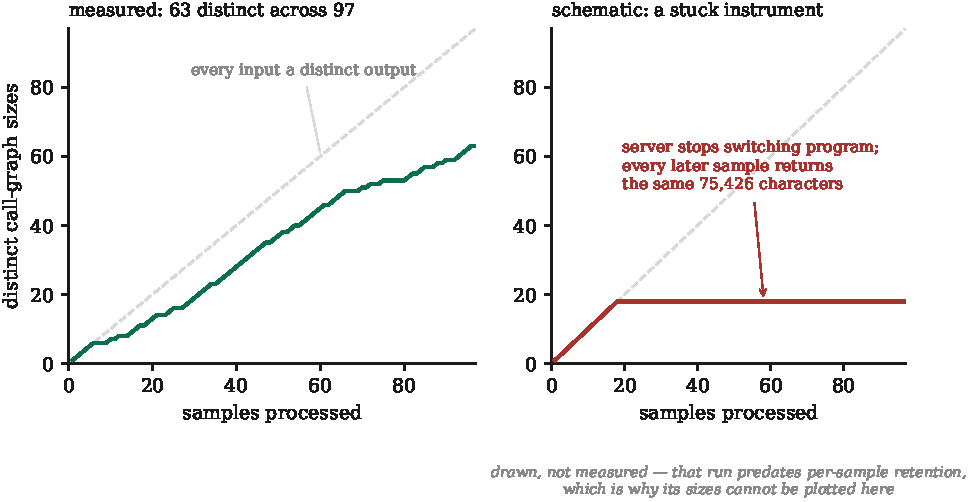
\includegraphics[keepaspectratio,alt={Figure 4: the whole detector, drawn. Panel a) is a measured run, panel b) a schematic of a stuck instrument.}]{figures/fig1-output-cardinality.pdf}}
\caption{The whole detector, drawn. a) a measured run at \fact{cardinality-distinct-graphs} distinct call-graph sizes across \fact{cardinality-samples} samples, b) a schematic of a stuck instrument. Panel b is drawn rather than measured because the run it depicts predates the per-sample retention these failures caused us to adopt, so its sizes no longer exist to plot.}
\label{fig:cardinality}
\end{figure}

The price is a completed study. A seven-year \fact{drift-n}-sample temporal-drift analysis ran the
full pipeline per sample against a long-lived server never restarted between samples, which is M2's
precondition exactly, and whether it was affected cannot be determined because its per-sample
outputs were not retained. The withdrawal is caused by the defect plus the inability to re-ask the
question afterwards.
